\documentclass[12pt]{article}

\usepackage{amsmath, amssymb}
\usepackage{tabularx}
\usepackage{array}
\usepackage{geometry}
\usepackage{tikz}
\usepackage{pdflscape}

\geometry{margin=2cm}

\renewcommand{\arraystretch}{1.6}

\begin{document}

\begin{landscape}

\begin{center}
{\LARGE \textbf{Catálogo de Distribuciones de Probabilidad}}
\end{center}


\vspace{0.7cm}

\begin{center}
\begin{tabular}{|c|c|c|c|c|c|c|}
\hline
Distribución & Nom. & Función & $E[X]$ & $Var(X)$ & $M_X(t)$ & Gráfica \\
\hline

\multicolumn{7}{|c|}{\textbf{Distribuciones Discretas}} \\
\hline

Binomial & $B(n,p)$ & $\binom{n}{x}p^x(1-p)^{n-x}$ 
& $np$ & $np(1-p)$ & $(1-p+pe^t)^n$ &
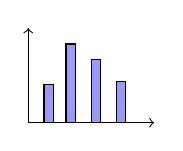
\begin{tikzpicture}[scale=0.4]
\draw[->] (0,0)--(4,0);
\draw[->] (0,0)--(0,3);
\foreach \x/\h in {0.5/1.2,1.2/2.5,2/2,2.8/1.3}
\draw[fill=blue!40] (\x,0) rectangle +(0.3,\h);
\end{tikzpicture}
\\
\hline

Poisson & $P(\lambda)$ & $\frac{e^{-\lambda}\lambda^x}{x!}$ 
& $\lambda$ & $\lambda$ & $e^{\lambda(e^t-1)}$ &
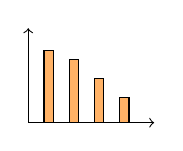
\begin{tikzpicture}[scale=0.4]
\draw[->] (0,0)--(4,0);
\draw[->] (0,0)--(0,3);
\foreach \x/\h in {0.5/2.3,1.3/2,2.1/1.4,2.9/0.8}
\draw[fill=orange!60] (\x,0) rectangle +(0.3,\h);
\end{tikzpicture}
\\
\hline

Geométrica & $Geom(p)$ & $(1-p)^{x-1}p$ 
& $\frac{1}{p}$ & $\frac{1-p}{p^2}$ & $\frac{pe^t}{1-(1-p)e^t}$ &
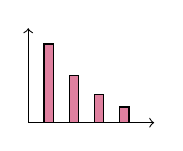
\begin{tikzpicture}[scale=0.4]
\draw[->] (0,0)--(4,0);
\draw[->] (0,0)--(0,3);
\foreach \x/\h in {0.5/2.5,1.3/1.5,2.1/0.9,2.9/0.5}
\draw[fill=purple!50] (\x,0) rectangle +(0.3,\h);
\end{tikzpicture}
\\
\hline

Uniforme Discreta & $U\{1,\dots,n\}$ & $\frac{1}{n}$ 
& $\frac{n+1}{2}$ & $\frac{n^2-1}{12}$ 
& $\frac{e^t(1-e^{nt})}{n(1-e^t)}$ &
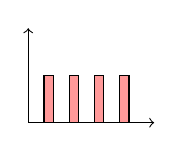
\begin{tikzpicture}[scale=0.4]
\draw[->] (0,0)--(4,0);
\draw[->] (0,0)--(0,3);
\foreach \x in {0.5,1.3,2.1,2.9}
\draw[fill=red!40] (\x,0) rectangle +(0.3,1.5);
\end{tikzpicture}
\\
\hline

\multicolumn{7}{|c|}{\textbf{Distribuciones Continuas}} \\
\hline

Normal & $N(\mu,\sigma^2)$ 
& $\frac{1}{\sigma\sqrt{2\pi}}e^{-\frac{1}{2}(\frac{x-\mu}{\sigma})^2}$ 
& $\mu$ & $\sigma^2$ & $e^{\mu t + \frac{\sigma^2 t^2}{2}}$ &
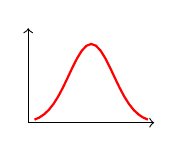
\begin{tikzpicture}[scale=0.4]
\draw[->] (0,0)--(4,0);
\draw[->] (0,0)--(0,3);
\draw[red, thick, domain=0.2:3.8] plot (\x,{2.5*exp(-(\x-2)^2)});
\end{tikzpicture}
\\
\hline

Exponencial & $Exp(\lambda)$ 
& $\lambda e^{-\lambda x}$ 
& $\frac{1}{\lambda}$ & $\frac{1}{\lambda^2}$ 
& $\frac{\lambda}{\lambda - t}$ &
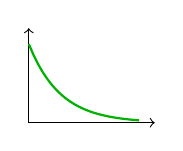
\begin{tikzpicture}[scale=0.4]
\draw[->] (0,0)--(4,0);
\draw[->] (0,0)--(0,3);
\draw[green!70!black, thick, domain=0:3.5] plot (\x,{2.5*exp(-\x)});
\end{tikzpicture}
\\
\hline

Uniforme & $U(a,b)$ 
& $\frac{1}{b-a}$ 
& $\frac{a+b}{2}$ & $\frac{(b-a)^2}{12}$ 
& $\frac{e^{tb}-e^{ta}}{t(b-a)}$ &
\begin{tikzpicture}[scale=0.4]
\draw[->] (0,0)--(4,0);
\draw[->] (0,0)--(0,3);
\draw (1,1.8)--(3,1.8);
\draw[dashed] (1,0)--(1,1.8);
\draw[dashed] (3,0)--(3,1.8);
\end{tikzpicture}
\\
\hline

\end{tabular}
\end{center}

\end{landscape}

\end{document}